\chapter{Literature Review}

This chapter reviews existing literature related to blockchain-based citizen reporting systems and their application in local governance. The reviewed studies focus on digital citizen reporting platforms, blockchain-enabled governance solutions, permissioned blockchain architectures, consensus mechanisms, decentralized storage techniques, and \ac{AI}-assisted content moderation approaches. In here we examine these areas to understand the design and technological foundation of the proposed system.

\section{Digital Citizen Reporting and e-Governance Systems}

Electronic governance (e-governance) is using the information and communication technologies to provide government services. This includes the support of government to citizens (G2C), government to business (G2B) , government to agencies (G2A) etc. By utilizing the e-governance platforms, everyone can gain access to whole range of public services. Additionally citizens can submit complaints and participate in governance decision making process. \cite{9587836}.

Digital citizen reporting system is one of the many use case of e-governance. "FixMyStreet" is a a such existing platform. It enable citizens to report issues for different issue categories. Sanitation, Traffic and Public Safety are some examples. Previous studies shows that these kind of systems improve governance administrative efficiency, civic participation and also they increase the transparency.\cite{oliveira2020smartcities}.

Even though there are many benefits of digital citizen reporting in local governance as described earlier, most of them still use centralized server based architecture. This centralized approach have its own limitations and  disadvantages. Susceptibility to data tempering, lack of transparency are the main problems that impact heavily on public trust. In addition to that, mandatory identity disclosure is discouraging public participation on this kind of reporting systems. Therefore these problems motivate the findings of new decentralized, transparent and immutable architectures that still preserve user privacy with accountability.





\section{Blockchain for Local Governance Applications}

Blockchain is a technology that has been popular for its ability to have an immutable, transparent and decentralized ledger for public data. Hence, its a transformative tool for e-governance to address the problems that existing implementations had. The Blockchain allow us to verify the immutability of the records, so its suitable for governance applications where the trust and the accountability is crucial. \cite{hamill2018blockchain}, \cite{goswami2020egovernance}.

Blockchain based land registry system implemented in Cook Country, Illinois is a one real world example of the applicability of blockchain in local governance. They aim to reduce the property fraud by consolidating historical ownership records into a verifiable block in the blockchain. Similar to that Delaware has taken initiative to explore the use of smart contracts that's enable real time asset tracking and automate business fillings. This improves the regulatory compliance and oversights \cite{goswami2020egovernance}.

In addition to administrative efficiency, blockchain has been utilized for citizen centric services, such as secure digital identity management. Estonia has taken a initiative to integrate blockchain across healthcare, taxation and even electronic voting systems. So this can provide a mathematically verifiable audit trail for government data. MyPass project in Austin and the World Food Program's building blocks initiative also use Blockchain technology under the hood to manage encrypted identity and transaction records \cite{hamill2018blockchain}.

Despite the advancements in the blockchain base applications, existing literature highlights the challenges of adoption in governance. Scalability constraints, privacy concerns related to identity data, performance overhead and also the need of the legislative and institutional reforms are  some examples. These factors needs to be addressed by carefully selecting blockchain architectures and consensus mechanisms before implementing systems for frequent citizen interactions.

\section{Blockchain-Based Citizen Reporting and Complaint Management Systems}

The traditional centralized platforms have data integrity issues, transparency issues and trust issues when it comes to citizen reporting. Past works also indicates that centralized complaint registries often have single point of failures , delayed responses and public mistrust. Therefore blockchain integrated reporting services can be used to mitigate those issues. 

A blockchain based police complaint management system has proposed by Pratheeba \cite{pratheeba_blockchain_police_complaint} contains a modular architecture. It's include security, blockchain, web interface and a hybrid cloud storage. This system ensure immutability of complaint records by cryptographic hash linking. And also it utilize RSA based encryption to restrict the access only to authorized personnel. In Addition to that, Pratheeba used a Natural Language Processing (NLP) techniques to automatically categorize complaints in the system based on their priorities. 

\begin{figure}[h!]
    \centering
    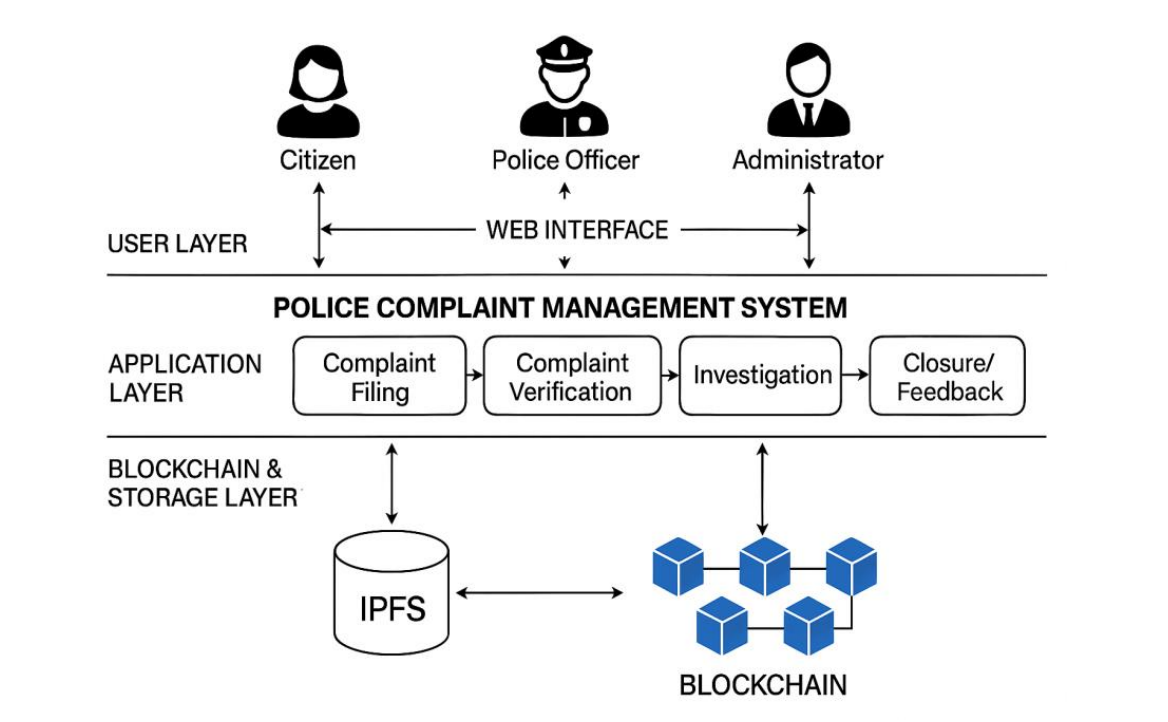
\includegraphics[width=0.95\textwidth]{figures/system-architecture-police-complaint-system.png} % Replace with your image file
    \caption{System Architecture of the Police Complaint Management System.\cite{manjula2025decentralized}}
    \label{fig:complaint-managment-system-architecture}
\end{figure}


A three tier architecture for decentralized complaint management framework has proposed by Manjula \cite{manjula2025decentralized} is shown in the Figure \ref{fig:complaint-managment-system-architecture}. The three layers are web based presentation layer, a business logic layer and finally a blockchain data layer. This system has a role based access control method to involve multiple stakeholders. Citizens, Law enforcement authorities and judicial bodies are some of them. More importantly this system has a immutable storage for multimedia evidences. Intelligent complaint assignment based on workloads, automatic escalation mechanism are some of the key features of the framework. The experimental evaluations shows that a significant reductions in complaint processing time. The successful detection of data tampering also archived by blockchain verification.

In literature, existing blockchain based complaint management systems shows some improvements in transparency and administrative efficiency. But most of them are domain specific. They primarily target law enforcement or isolated governance functions. In addition to that several platforms still rely on centralized architectures. Only a limited attention is given for implementing a community assisted validation, for privacy preserving reporting mechanisms and efficient handling of multimedia evidences. Therefore these limitations highlight the need for a generalized reporting framework for local governance.
\section{Permissioned Blockchains and \ac{PoA} Consensus Mechanisms}

Based on the participation and access control blockchain network can be classified in to two categories.  \cite{und2026commledger}. They are permissionless architecture (public) and permissioned architecture. Bitcoin and Early Ethereum networks are permissionless blockchains. They allowed unrestricted participation and relyed on consensus mechanism like \ac{PoW} or Proof of Stake (\ac{PoS})\cite{mdpi2023survey}. These architectures and consensus mechanisms emphasized decentralization among participants. But they often suffer from the high latency of the network, limited throughput and unpredictable transaction costs due to congestion. These problems make the traditional permissionless PoW or PoS consensus mechanisms unsuitable for governance and crowdsourced applications\cite{arxiv2024performance}.

While permissionless blockchains are unsuitable for governance related applications, permissioned blockchains restrict the network participation to authorized entities. This enables more efficient consensus mechanisms and greater control over governance data \cite{und2026commledger}. This known identities of participants allow permissioned systems to achieve higher performance. And support the regulatory compliances, data privacy and structured governance models as well cite{mdpi2023unleashing}.

Other than \ac{PoW} and \ac{PoS} consensus mechanisms, \ac{PoA} offer significant advantages over permissioned blockchains. \ac{PoW} requires energy intensive computation. \ac{PoS} relies on the economic stake and introduce wealth centralization risks. But on the other hand \ac{PoA} depends on the identity and the reputation of pre approved validators\cite{researchgate2020survey}, \cite{zebpay2026poa}. Therefore this \ac{PoA} consensus mechanism enables high transaction throughput and low latency. And also it mitigate the issues such as the "nothing at stake" problem by off chain legal and reputational accountability \cite{echo2026poa}, \cite{grokipedia2026poa}.

The government systems should have accountability, performance predictability and data confidentiality. The \ac{PoA} is well suited consensus mechanism for that \cite{onekey2026poa}. By using \ac{PoA} we can have the ability to identify and regulate validator entities to align blockchain operations. It's because we have the existing legal frameworks that ensure institutional responsibility. Hence, can avoid malicious behavior \cite{hep2023governance}. In Addition to that PoA avoids the indeterministic transaction fees and support controlled validation environments. This make them viable for handling sensitive governmental data under regulatory constraints\cite{zebpay2026poa},\cite{mdpi2023unleashing}. As a result, \ac{PoA} emerges as a practical consensus mechanism for permissioned blockchain-based reporting systems in local governance contexts.


\section{Smart Contracts for Public Issue Management and Opinion Polling}

In governance systems, to improve the transparency, efficiency and citizen participation, smart contracts have been explored as the good mechanism. Smart contracts can automate the governance rules and incentives by immutable code. It can support models like civic intelligence governance (CIG). In CIG, citizen engagement is encouraged through on chain participation and token based incentives\cite{MDPI_2023_CivicIntelligence}. Literature shows that approaches like CIG can improve participation rates and knowledge sharing while reducing relances on centralized intermediaries. In the context of multi organizational governance smart contracts also been used within dual blockchain architectures. This method separates transaction data from contract logic. It balance the transparency and privacy in Government to Government and Business to Business processes\cite{IEEE_2021_SmartCon}.

% Smart contracts also help  business process reengineering in governance processes by directly embedding policy rules into the executable logic. Also the smart contracts help to do the tendering processes and public procurement, automate bid submission, evaluation, and contract execution by making these processes with zero chances for corruption and also increasing the accountability \cite{IEEE_2021_SmartCon}, \cite{GovernanceNow_2023_SmartContractsToolkit}, \cite{AICERTs_2023_FutureOfGovernance}. Also Similar benefits can be seen in blockchain based land registry systems by enabling immutable property records, automated ownership transfers and enforcement of land use policies. So again this reduces the
% fraud and inefficiencies in administratives \cite{ResearchGate_2020_LandRegistry}, \cite{MDPI_2023_NamibianLandRegistration}.

Smart contracts also support business processes in governance by embedding policy rules directly into executable logic. Bid submission, evaluation and contract execution are some of the use cases in the public procurement and tendering processes that smart contract hold its value. It also reduce the oppertunities for corruption and increase the accountability\cite{IEEE_2021_SmartCon}, \cite{GovernanceNow_2023_SmartContractsToolkit}, \cite{AICERTs_2023_FutureOfGovernance}. Similar benefits are observed in the blockchain based land registry systems. Smart contracts have enable immutable property records automated ownership transfers and enforcement of land use policies. This has reduced fraud and administrative inefficiencies\cite{ResearchGate_2020_LandRegistry}, \cite{MDPI_2023_NamibianLandRegistration}.

% If we consider voting and opinion polling, blockchain based systems make sure the security and transparency is protected by ensuring immutability and verifiability of votes while preserving voter anonymity \cite{ResearchGate_2024_ScalableEVoting}, \cite{IEEE_2024_BPVot}. Advanced mechanisms like Quadratic Voting and blockchain enabled participatory budgeting increases the citizen involvement in decision making. They allow more visibility in preference representation and transparent allocation of public resources \cite{ResearchGate_2021_QuadraticVoting}, \cite{UPSpace_2022_ParticipatoryBudgeting}. Eventhough there are many advantages like that, existing studies also highlight some challenges related to scalability, privacy, and system complexity. Particularly when deploying voting and polling solutions for large and diverse populations \cite{ResearchGate_2024_ScalableEVoting}, \cite{JournalOfCybersecurity_2020_BlockchainVoting}.

In the context of voting and opinion polling, smart contracts offer enhanced security, transparency, immutability and verifiability inherited from blockchain\cite{ResearchGate_2024_ScalableEVoting}, \cite{IEEE_2024_BPVot}. There are advance mechanisms such as Quadratic Voting and also blockchain enabled participatory budgeting. Those mechanisms further extend citizen involvement in decision making. It have expressive preference representation and transparent allocation of public resources\cite{ResearchGate_2021_QuadraticVoting}, \cite{UPSpace_2022_ParticipatoryBudgeting}. In addition to these advantages, there exists some challenges related to scalability, privacy and system complexity when deploying voting and polling systems to large and diverse populations\cite{ResearchGate_2024_ScalableEVoting}, \cite{JournalOfCybersecurity_2020_BlockchainVoting}.


\section{User Interfaces for Blockchain-Based e-Gover\\nance Applications}

User interfaces play a critical role in determining the accessibility and adoption of blockchain based e-governance systems. In the traditional applications the user literacy is less important but in this conventional blockchain applications the user literacy is highly considered because of the blockchain concepts that are different from the traditional apps and it does make the users hard to understand and adopt. The literature consistently identifies usability and user experience challenges as major barriers to the adoption of decentralized applications for the general public. Particularly where security requirements conflict with established usability principles \cite{mdpi2025usercentric}, \cite{sonule2025uxweb3}. So the design of intuitive, inclusive, and responsive web interfaces is essential for enabling effective interaction between citizens, government officials, and the underlying blockchain infrastructure.

\subsection{Usability Challenges in Decentralized Governance Systems}

Decentralized applications are fundamentally different from traditional web systems due to its architectural characteristics. Blockchain based systems have asynchronous transactions, immutable records, and cryptographic identity management. They can create friction for users who are used to centralized platforms. Studies highlight a significant usability gap in Web3 applications because of the concepts like transaction finality, gas fees, and private key ownership which are difficult for non technical users to understand and manage  \cite{mdpi2025usercentric}, \cite{sonule2025uxweb3}.

\subsection{Identity Management and Cognitive Load}

One of the most critical usability barriers is wallet based identity management. The reason is user identity is tied to cryptographic key pairs instead of institution managed accounts In decentralized systems. Research shows that the responsibility of safeguarding private keys and the unrecoverble key loss red ce the user participation. Specially in general public where inclusivity is essential \cite{sonule2025uxweb3}, \cite{ramotion2026uiux}, \cite{fintechweekly2025usability}.  

The literature further shows that concepts such as self-sovereign identity and identity management remain poorly understood by most users. Studies report unsafe practices and misunderstanding of recovery mechanisms when users are presented with seed phrases or key-based authentication \cite{oup2022governance}, \cite{fraunhofer2026usability}. These findings motivate the need for interface-level abstractions that preserve blockchain security while reducing cognitive load for citizens and officials.

\subsection{Transaction Latency and User Feedback}

Blockchain transactions are inherently asynchronous with confirmation times dependent on network conditions and consensus protocols. This latency can lead to confusion among  the users because of the system status problems and users can determine those as system failures \cite{sonule2025uxweb3}. The literature recommends to use an optimistic user interface pattern, where user actions are acknowledged immediately while blockchain confirmation occurs in the background.  

As advanced design solutions, literature shows progressive status disclosure, distinguishing between off-chain receipt of a report and on-chain verification which allows users to track the lifecycle of an issue without being exposed to unnecessary low level blockchain details \cite{dzone2026blockchainai}, \cite{marian2025transparent}. Mechanisms like that are particularly relevant for issue reporting systems that require transparency and trust.

\subsection{Transaction Costs and Abstraction of Blockchain Complexity}

% Another significant usability challenge arises from transaction costs associated with public blockchains. The concept of gas fees and fluctuating costs is unfamiliar in public service contexts, where users expect free access to reporting platforms \cite{mdpi2025usercentric}. The literature strongly supports the use of gas abstraction techniques, such as meta-transactions, where backend relayer services submit transactions on behalf of users while preserving cryptographic intent verification \cite{sonule2025uxweb3}. This approach enables blockchain interaction without exposing citizens to economic or technical complexities.

A significant usability challenge coming from the blockchain is transaction cost that associated with public blockchains. And also the concepts of gas fees and fluctuating gas costs are very unfamiliar in public services context. Most of the time users expect free access to the reporting platforms\cite{mdpi2025usercentric}. The literature strongly suggest that the use of gas fee abstraction techniques. Meta Transactions is one of the example. In Meta, backend relayer services submit transactions on behalf of the user. Its achieved by preserving cryptographic intent verification\cite{sonule2025uxweb3}. Therefore this approach enable citizen to interact with blockchain without technical or economical complexities.


\subsection{Comparison with Centralized Reporting Platforms}

% Existing centralized platforms such as FixMyStreet and SeeClickFix provide valuable benchmarks for citizen reporting interfaces. Their success is attributed to intuitive map-based reporting, simple authentication mechanisms, and clear feedback loops that inform users about issue resolution progress \cite{king2012fixmystreet}, \cite{mysociety2026fixmystreet}. SeeClickFix further incorporates gamification mechanisms to encourage participation, although studies caution against over-financializing civic engagement \cite{seeclickfix2011democracy}.  

% In contrast, blockchain-based reporting platforms must reconcile these usability expectations with immutable data storage, decentralized identity, and transparent verification. The literature highlights the need for interface designs that visualize blockchain guarantees such as data integrity and auditability—using familiar metaphors rather than raw cryptographic representations \cite{adeyeye2025blockchain}, \cite {marian2025transparent}, \cite{nikonenko2025blockchain}.  

% Additionally, as multimedia evidence is central to citizen reporting, interfaces must integrate decentralized storage solutions such as InterPlanetary File System (\ac{IPFS}) in a seamless manner, ensuring that large media files are handled off-chain while their integrity is verifiably linked on-chain without exposing technical details to users \cite{mergel2012distributed}, \cite{pazos2024blockchain}.

FixMyStreet and SeeClickFIx are existing centralized platforms. Eventhough they are centralized, they provide a valuable benchmarks for crowdsource citizen reporting interfaces. Inituitive map based reporting, simple authentication mechanisms and clear feedback loops are the key characteristics that attributed to platform success\cite{king2012fixmystreet}, \cite{mysociety2026fixmystreet}.

With addition to that SeeClickFix further uses a gamification mechanism to encourage the users to participate in the system. In contrast, Even though the proposed application uses blockchain for reporting platform, it must retain the usability and the expectations of the users. The literature highlights the need of interface design such that gurantees the data integrity and auditability using familiar ui elements rather than cryptographic representations\cite{adeyeye2025blockchain}, \cite {marian2025transparent}, \cite{nikonenko2025blockchain}.  

% \subsection{Trust, Anonymity, and Transparency in Interface Design}

% For privacy-preserving reporting systems, user trust depends not only on protocol guarantees but also on how those guarantees are communicated through the interface. Research on privacy-focused reporting systems emphasizes that users must clearly understand that anonymity is mathematically enforced rather than institutionally promised \cite{lin2023prirpt}. Visual explanations and contextual cues have been shown to improve trust and comprehension more effectively than generic security labels \cite{fraunhofer2026usability}.  

% Similarly, transparency mechanisms such as verification badges, audit timelines, and status indicators help bridge the gap between blockchain-level transparency and human interpretability, enabling users to track issue resolution without interacting directly with block explorers or raw ledger data. \cite{marian2025transparent}, \cite{nikonenko2025blockchain}

\subsection{Accessibility and Inclusivity Considerations}

Inclusivity is a fundamental requirement for e-governance systems. According to \cite{bertrand2023connected}, it can be seen that poorly designed blockchain interfaces may digitally divide users. Also it may favor crypto-literate users excluding vulnerable populations. To reduce this issue, literature suggests mobile first design approaches. Furthermore, lightweight client architectures, effiecient bandwidth synchronization can used to support access in resource limited environments.  \cite{shahin2025towards}.  

% The literature warns that poorly designed blockchain interfaces risk exacerbating the digital divide by favoring crypto-literate users and excluding vulnerable populations \cite{bertrand2023connected}. To mitigate this risk, studies advocate mobile-first design approaches, lightweight client architectures, and bandwidth-efficient synchronization to support access in resource-constrained environments \cite{shahin2025towards}.  

% Furthermore, low-code and no-code development platforms are emerging as viable solutions for enabling local governments to deploy and customize reporting interfaces without extensive blockchain expertise, supporting scalability and adaptability across different governance contexts \cite{quixy2025citizen}. These approaches align with the objective of developing user-friendly interfaces that facilitate broad participation and effective interaction with blockchain-based reporting systems.

\section{AI-Based Content Moderation in Civic Reporting}

Since blockchain is inheritably immutable its introduce a unique challenge for content moderation in a civic reporting system. In a centralized platforms, administrators can remove or edit inappropriate content. But in a decentralized blockchain based system data cannot be altered once confirmed \cite{tencentcloud2025moderation}. While immutability strengthens transparency and accountability, it also raises the risk of permanently storing harmful, illegal, or misleading content. Therefore the literature focuses the need for pre moderation strategies to prevent unsuitable content from being recorded on chain or to limit its visibility after publication \cite{dzone2026blockchainai}.

\subsection{Need for Automated Content Moderation}

Civic reporting platforms are susceptible to several forms of misuse that can compromise system reliability and public trust. Automated spam submissions, the submission of malicious or legally sensitive content, and deliberate dissemination of false or misleading reports are some of the common issues \cite{wani2024ai}, \cite{gosztonyi2024theory}, \cite{kolluri2025aipowered}. Manual moderation is impractical for above situations. Since the reporting system is large latency, human bias, and operational costs can occur. Furthermore it reintroduces the centralized control structure that blockchain system is aim to minimize. 

Therefore the literature supports AI assisted moderation as a scalable and  efficient approach for filtering content before its permanently recorded. It maintain the acceptable levels of decentralization \cite{mohammadi2025ai}, \cite{goundar2025blockchain}.

\subsection{Architectural Approaches for AI Blockchain Integration}

Due to the computational and storage limitations of blockchain platforms, AI-based moderation cannot be performed directly on chain. Off chain processing combined with on chain verification identified by existing researches as most practical approach\cite{goundar2025blockchain}, \cite{kader2024enhancing}.  

In this approach, reported content is first analyzed by AI models hosted off chain infrastructure or decentralized compute networks. The outcome of this analysis is a validation decision or a trust score. This outcome then submitted to the blockchain as a cryptographic proof or oracle response. Next the smart contracts verify those results before accepting the report. It will ensure that only the content meeting predefined policies are recorded on chain. BlockCITE is a example framework demonstrate how this separation preserves blockchain integrity while avoiding excessive on chain computation \cite{li2025blockcite}.

\subsection{\ac{AI} Oracles and Decentralized Oracle Networks}

Oracles are trusted intermediaries that connect on chain and off chain. In here the \ac{AI} oracles provides the computational results to smart contracts. Instead of simply retrieving external data to the blockchain, \ac{AI} oracle perform content classification and verification tasks. Then it returns the structured results to the blockchain \cite{kava2024aipowered}, \cite{zintusart2025empirical}.  

There can be a risk of oracle bias or failure. To minimize the risk a decentralized oracle networks aggregate outputs from multiple independent \ac{AI} nodes and determine consensus outcomes. This model reduces reliance on a single \ac{AI} system. Therefore it improves te robustness by requiring agreement among multiple validators\cite{zintusart2025empirical}, \cite{codezeros2025aipowered}.

\subsection{Techniques for Content Analysis}

\ac{AI}-based moderation techniques vary based on the type of submitted content. \ac{NLP} models are widely used to detect spam, hate speech and misinformation for text based reports. Studies report high accuracy when combining deep learning models with semantic embeddings. It makes them suitable for filtering large volumes of text submissions prior to blockchain recording \cite{wani2024ai}.  

For image based reports computer vision models are used to identify inappropriate contents. However recent advances in generative AI increase the risk of fabricated images. This literature proposes a hybrid verification pipeline that combine cryptographic provenance mechanisms with \ac{AI}-based image analysis. This ensue that the submitted media is both authentic and contextually valid \cite{prasad2024blockchain}.

\subsection{Hybrid Human AI Moderation Models}

AI enable the scalable moderation. But it may struggle with contextual interpretation and edge cases. Because of that many studies advocate hybrid moderation models. In those models AI performs initial filtering and prioritization, while human reviewers handle disputed or ambiguous cases \cite{mohammadi2025ai}, \cite{kumar2025hybrid}. 

Decentralized community based moderation further complement this approach. The models using community annotation systems, allow users or designated validators to challenge AI decisions during predefined review periods. In Addition to that dispute resolution handled by transparent governance mechanisms \cite{dzone2026blockchainai}, \cite{kae2025research}. Therefore these strategies reduce the reliance on central authority while maintain the accountability.

\subsection{Ethical Considerations and Content Permanence}

Ethical concerns are crucial when implementing systems by integrating AI driven moderation systems. The algorithmic bias and the accountability are the highlights in the literature. Biased training data can lead to unfair rejection of legitimate reports\cite{chase2024ai}. To minimize this risk explainable AI mechanisms are recommended. This enable users to understand the moderation decision and resubmit corrected reports \cite{mounika2024integrated}. 

Finally, the issue of “toxic immutability” remains a critical challenge for blockch\\ain-based systems. To resolve this issue its suggested that to use a off chain storage systems like IPFS. If the content is later identified as illegal or harmful, it can removed from the off chain storage. But can preserve the immutable audit trail by recording it on the blockchain\cite{prasad2024blockchain}. The transparency, legal compliance and ethical responsibility can be balanced by this approach.

% \section{Trustworthiness and Reputation Models in Crowdsourced Systems}

% A fundamental challenge in blockchain-based civic reporting systems is enabling anonymous participation while maintaining trust in submitted reports. Traditional reporting systems derive trust from user identity; however, decentralized and privacy-preserving systems must instead evaluate trust based on user behavior and collective validation. The literature addresses this challenge through reputation and trustworthiness models that decouple identity from reliability, allowing users to remain anonymous while their contributions are evaluated objectively.

% \subsubsection{Concept of Trustworthiness in Crowdsourced Reporting}

% Trustworthiness in crowdsourced reporting is commonly defined as a multi-dimensional concept encompassing data quality, consistency, and contributor behavior \cite{gheyas2025establishing}. Data quality refers to the accuracy and completeness of submitted information, data reliability is assessed through agreement with other reports or historical patterns, and contributor credibility reflects the past behavior of the reporting entity. Together, these dimensions allow systems to assess reports without requiring real-world identity disclosure.

% \subsubsection{Anonymous Reputation Mechanisms}

% To support anonymity while preventing abuse, several reputation mechanisms have been proposed. Identity-bound pseudonymity is a widely cited approach, where a user possesses a verified root identity but interacts with the system using unlinkable pseudonyms \cite{androulaki2008reputation}. Reputation is cryptographically linked to the root identity, ensuring accountability while preserving privacy. This approach mitigates Sybil attacks, as malicious behavior under one pseudonym affects the user's overall reputation, limiting repeated abuse \cite{androulaki2008reputation}, \cite{kaafarani2018anonymous}.

% \subsubsection{Blockchain-Based Reputation Frameworks}

% The PriRPT framework is a notable example of a privacy-preserving reporting system that integrates anonymous credentials and reputation mechanisms \cite{lin2023prirpt}. Users register with a trusted authority and subsequently submit reports using derived anonymous credentials. Verified reports are rewarded without linking the reporter’s identity to the reward, preserving unlinkability. By employing optimized cryptographic schemes, PriRPT demonstrates feasibility for mobile-based civic reporting applications.

% Similarly, the Block-CITE framework proposes a dual-blockchain architecture to separate reporting tasks from reputation management \cite{li2025blockcite}. One chain stores report data, while a second chain maintains reputation scores. This separation improves scalability and allows reputation updates without congesting the primary reporting ledger. Reputation is incremented based on report validation outcomes, reinforcing honest participation while maintaining privacy.

% \subsubsection{Peer Validation and Consensus-Based Trust}

% In decentralized environments, trust is often established through peer validation mechanisms. Reports may be verified by nearby users or relevant stakeholders, leveraging the “wisdom of the crowd” principle \cite{hasan2023privacy}. Consensus-based approaches reward users whose validations align with the majority, while penalizing inconsistent behavior. To prevent manipulation, many systems employ weighted voting schemes where votes are scaled by reputation scores, ensuring that trusted contributors have greater influence \cite{leonardos2022weighted}, \cite{aluko2021proof}, \cite{hewa2025repuchain}.

% \subsubsection{Algorithmic Trust and Reputation Scoring}

% Trust scores are typically computed using mathematical models that adapt over time. Subjective logic models represent trust as a combination of belief, disbelief, and uncertainty, allowing nuanced decision-making in uncertain environments \cite{zupancic2019data} ,\cite{fu2022bfcri}. Other approaches use growth functions and time-decay mechanisms to ensure that reputation is earned gradually and must be maintained through consistent honest behavior \cite{zupancic2019data}, \cite{das2014re3}. These models reduce the risk of reputation manipulation and ensure responsiveness to recent behavior.

% \subsubsection{Trust in Mobile Crowdsensing Contexts}

% For automated or sensor-based reports, such as those generated by mobile devices, trust evaluation must account for device reliability and environmental variability. Probabilistic models compare sensor readings against nearby observations to detect anomalies or faulty data \cite{zupancic2019data}, \cite{ali2020blockchain}. Additionally, location verification techniques, including proof-of-location protocols, are used to ensure that reports originate from the claimed physical location, preventing fraudulent submissions \cite{albilali2024blockchain}.

% Overall, the literature demonstrates that combining anonymous reputation systems, peer validation, and adaptive trust models enables reliable crowdsourced reporting without compromising user privacy. These approaches directly inform the design of blockchain-based community reporting platforms that aim to balance anonymity, accountability, and data integrity.


% % \subsection{Trustworthiness and Reputation Models in Crowdsourced Systems}

% % The core value proposition of a blockchain-based reporting system is that it allows for anonymous yet trusted participation. This presents a seeming paradox: how can a system trust a report if the source is unknown? In traditional systems, trust is transitive through identity (I trust User X, therefore I trust their report). In anonymous decentralized systems, trust must be derived from behavior and consensus. The literature resolves this through Reputation Systems and Trustworthiness Evaluation Models that dissociate identity (who you are) from reputation (how reliable you have been).

% % \subsubsection{Defining Trustworthiness in Crowdsourcing}

% % Trustworthiness in this context is a composite metric comprising three dimensions \cite{gheyas2025establishing}:  

% % \begin{enumerate}
% %     \item Data Quality: Is the data accurate, complete, and formatted correctly? (Objective verification).
% %     \item Data Reliability: Is the data consistent with other observations and historical trends? (Consensus verification). 
% %     \item Contributor Credibility: Does the user have a history of honest contributions? (Reputation).  
% % \end{enumerate}

% % \subsubsection{Mechanisms for Anonymous Reputation}

% % To evaluate trustworthiness without revealing identity, researchers have developed sophisticated cryptographic and algorithmic frameworks that allow a user to prove they are "reputable" without proving "who" they are.

% % \subsubsection{ Identity-Bound Pseudonymity}

% % A key innovation is the "Identity-Bound Reputation System" \cite{androulaki2008reputation}. In this model, a user has a real identity (e.g., a master key registered with a government authority) but interacts with the system using disposable pseudonyms. The reputation is mathematically linked to the master identity, but the link is hidden from the public .

% % \begin{itemize}
% %     \item Mechanism: When a user submits a report, they generate a Zero-Knowledge Proof (ZKP) that attests: "I am a member of the set of registered citizens, and my reputation score is above Threshold X," without revealing which member they are.
% %     \item Unlinkability: This prevents "Sybil attacks" (one user creating multiple fake accounts to boost a rating or spam the system) because the reputation is tied to a singular, verifiable root identity. If a user acts maliciously under one pseudonym, the penalty propagates to their master reputation, affecting all future pseudonyms \cite{androulaki2008reputation} \cite{kaafarani2018anonymous}. 
% % \end{itemize}

% % \subsubsection{The "PriRPT" Framework}

% % The PriRPT (Practical blockchain-based Privacy-Preserving Reporting System) is a prominent example in the literature that specifically addresses this challenge \cite{lin2023prirpt}. It integrates Keyed-Verification Anonymous Credentials (KVAC) and Structure-Preserving Signatures on Equivalence Classes (SPS-EQ).

% % Workflow:

% % \begin{enumerate}
% %     \item Registration: User registers with a trusted authority (TA) and receives a credential.
% %     \item Reporting: User submits a report signed with a derived credential. The signature proves validity but not identity.
% %     \item Rewarding: If the report is verified (e.g., leads to a fix), the system issues a reward token. The user can claim this token anonymously using the SPS-EQ scheme, breaking the link between the report submission and the reward payout address.
% %     \item Efficiency: By replacing general-purpose ZKPs with optimized signature schemes (SPS-EQ), PriRPT reduces the computational overhead, making it feasible for mobile devices, which is a critical constraint for citizen reporting apps \cite{lin2023prirpt}. 
% % \end{enumerate}

% % \subsubsection{The "Block-CITE" Framework}

% % Block-CITE proposes a dual-blockchain architecture to separate the task (the report) from the reputation (the trust score) to enhance scalability and privacy \cite{li2025blockcite}. 

% % \begin{itemize}
% %     \item TaskChain: Records the details of the crowdsourcing task (e.g., the report, evidence, and timestamps).
% %     \item RepuChain: Records the reputation scores of the participants.
% %     \item Interaction: Reputation is updated based on the outcome of the task. If a report is validated by the government or peers, the reputation score in RepuChain is incremented via a smart contract. This separation ensures that frequent reputation updates do not clutter the TaskChain, and allows for different privacy settings on each chain \cite{li2025blockcite}.
% % \end{itemize}

% % \subsubsection{Peer Validation and "Wisdom of the Crowd"}

% % In the absence of a central validator, the system must rely on peer validation. This is often modeled using Game Theory and Weighted Voting.

% % \begin{itemize}
% %     \item Schelling Points: In a decentralized voting game, users are incentivized to vote with the majority. If a user reports a pothole, and 10 neighbors also verify it (consensus), the report is deemed true. Users who vote with the consensus are rewarded; those who vote against are penalized. This mechanism assumes that the majority of citizens are honest \cite{hasan2023privacy}.  
% %     \item Weighted Voting: To prevent "mob rule" or attacks by bot farms, votes are weighted by reputation. A vote from a user with a high "Trustworthiness Score" counts significantly more than a new user's vote. This is detailed in "Proof of Reputation" (PoR) consensus mechanisms \cite{leonardos2022weighted}. The RepuChain protocol, for instance, uses a multi-factor reputation score (incorporating data validity, frequency, and latency) to elect leaders in the consensus process, ensuring that only trusted nodes validate data \cite{aluko2021proof} \cite{hewa2025repuchain}. 
% % \end{itemize}

% % \subsubsection{Algorithmic Trust Models}

% % Mathematical models are used to calculate the trust score dynamically, ensuring it reflects current behavior.

% % \begin{itemize}
% %     \item Subjective Logic: This approach models trust not as a single scalar number but as a "belief, disbelief, and uncertainty" triplet. It accounts for the fact that trust is subjective and transitive (User A might trust User B, but User C might not). This allows the system to filter reports based on a user's personal trust network \cite{zupancic2019data} \cite{fu2022bfcri}.   
% %     \item Gompertz Function: Some systems use the Gompertz function (an S-shaped curve) to model reputation growth—reputation is easy to lose (steep drop) but hard to gain (slow climb). This prevents users from rapidly "gaming" the system to achieve high trust scores before launching an attack \cite{zupancic2019data}. 
% %     \item Time-Decay: Reputation models often include a time-decay factor (EWMA - Exponentially Weighted Moving Average), ensuring that past good behavior doesn't grant permanent immunity to a user who starts acting maliciously. A user must maintain constant honest participation to keep a high score \cite{das2014re3}.
% % \end{itemize}

% % \subsubsection{Trust in Mobile Crowdsensing (MCS)}

% % For automated reports (e.g., a phone's accelerometer detecting a pothole automatically), trust models must account for device calibration and environmental noise.

% % \begin{itemize}
% %     \item Probabilistic Assessment: Trust is inferred from the statistical deviation of a user's data from the group mean. If one sensor reports a temperature of 100°C while ten others nearby report 25°C, the outlier is flagged as untrustworthy (faulty or malicious) \cite{zupancic2019data} \cite{ali2020blockchain}.   
% %     \item Location Proofs: "Proof of Location" protocols (using GPS + Wi-Fi triangulation logs stored on-chain) are critical to ensure that the user was actually physically present at the site of the report, preventing "armchair reporting" where users spoof locations to file fake reports \cite{albilali2024blockchain}.
% % \end{itemize}




% \section{Gaps in Literature}
% \subsection{Limited Integration of Privacy-Preserving Reporting and Blockchain}
% \subsection{Lack of AI-Assisted Moderation in Blockchain-Based Reporting Systems}
% \input{chapters/literature-review/gaps/2.2.3.section}
% \input{chapters/literature-review/gaps/2.2.4.section}
% \input{chapters/literature-review/gaps/2.2.5.section}

